\section{Homebrew Rules}
This section shall outline universal changes to this campaign's rules from combat, to travel and even roleplay.

\subsection{Travel}
Travel is broken up into three tiers of distance and cost.

\subsubsection{Nearby}
Travel to a place \textbf{Nearby}, will have at least \textbf{1 encounter}, \textbf{1 short rest} \textit{recommended} afterwards, though depending on how fast and what route you take, the encounter can be avoided and the number of resources can increase or decrease. 

\subsubsection{Far}
Travel to a place \textbf{Far} away, will have at least \textbf{2 encounters} and a \textit{required} \textbf{1 short rest} afterwards, though depending on how fast and what route you take, 1 of the 2 encounters can be avoided and the number of resources can increase or decrease.

\subsubsection{Very Far}
Travel to a place \textbf{Ver Far} away, will have at least \textbf{3 encounters}, \textbf{1 long rest} \textit{required} afterwards, though depending on how fast and what route you take, up to 2 encounters can be avoided and the number of resources can increase or decrease.

\subsection{Class Divergence}
Due to the restrictions of roleplay, It shall be allowed for certain classes to use \textbf{variant ability score modifiers} that fit the character better.

\subsubsection{Paladin}

The \textit{spellcasting modifier} for the paladin is \textbf{Wisdom} instead of \textbf{Charisma}.

\begin{DndReadAloud}
   As you will soon discover, this world is ripe with a feast of options and varieties of character flavour heard before only on the lips of a madman!
\end{DndReadAloud}

\begin{figure}
    \centering
    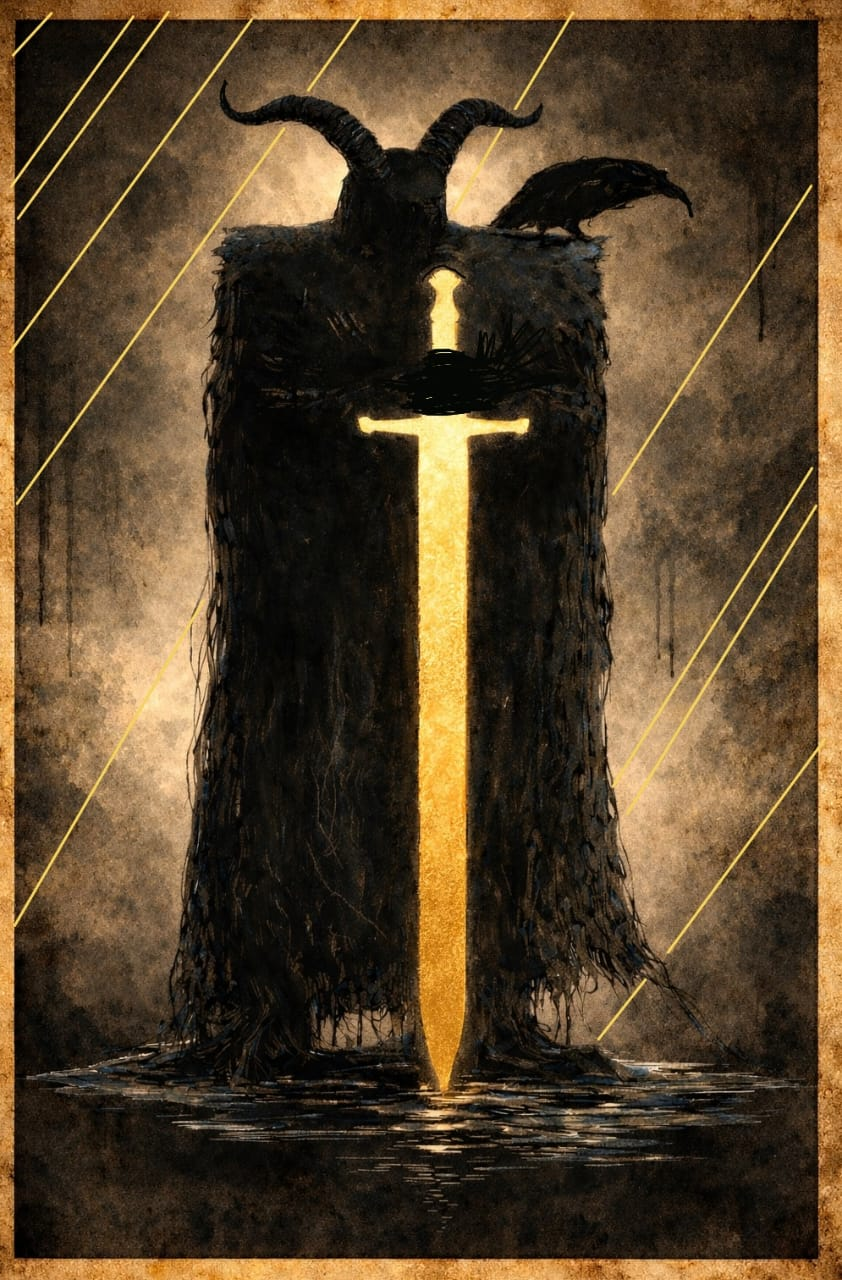
\includegraphics[width=0.7\linewidth]{Images/Black_Knight.jpeg}
    \label{fig:placeholder}
\end{figure}

\begingroup
\DndSetThemeColor[PhbMauve]
\begin{DndSidebar}{Black Knight}
\textit{}
\end{DndSidebar}
\endgroup

\subsubsection{Warlock}

The \textit{spellcasting modifier} for the base warlock is \textbf{Charisma}, though you may upon request choose to use \textbf{Intelligence instead}.

\subsubsection{Sorcerer}
The \textit{spellcasting modifier} for the base sorcerer is \textbf{Charisma}, though if you do not multiclass out of sorcerer, you may request to use \textbf{Constitution} instead.

\subsection{Critcal Rolls}
In the event that \textit{a\textbf{ Natural 20 }}or\textit{ \textbf{Natural 1}} is rolled, the \textbf{\textit{critical success or failure,}} respectively, gets an added effect determined by the \textit{Dungeon Master}.

\subsection{Hybrid Source-Material}
In this campaign, a joint use of the \textit{2014 PHB} and \textit{2024 PHB} shall be used to maximise the roleplaying potential of the adventurers and the world built within this vast tale.

\subsubsection{Species \& Backgrounds}
see the relevant chapter for the custom/adapted \textbf{species} available.

\begin{figure}
    \centering
    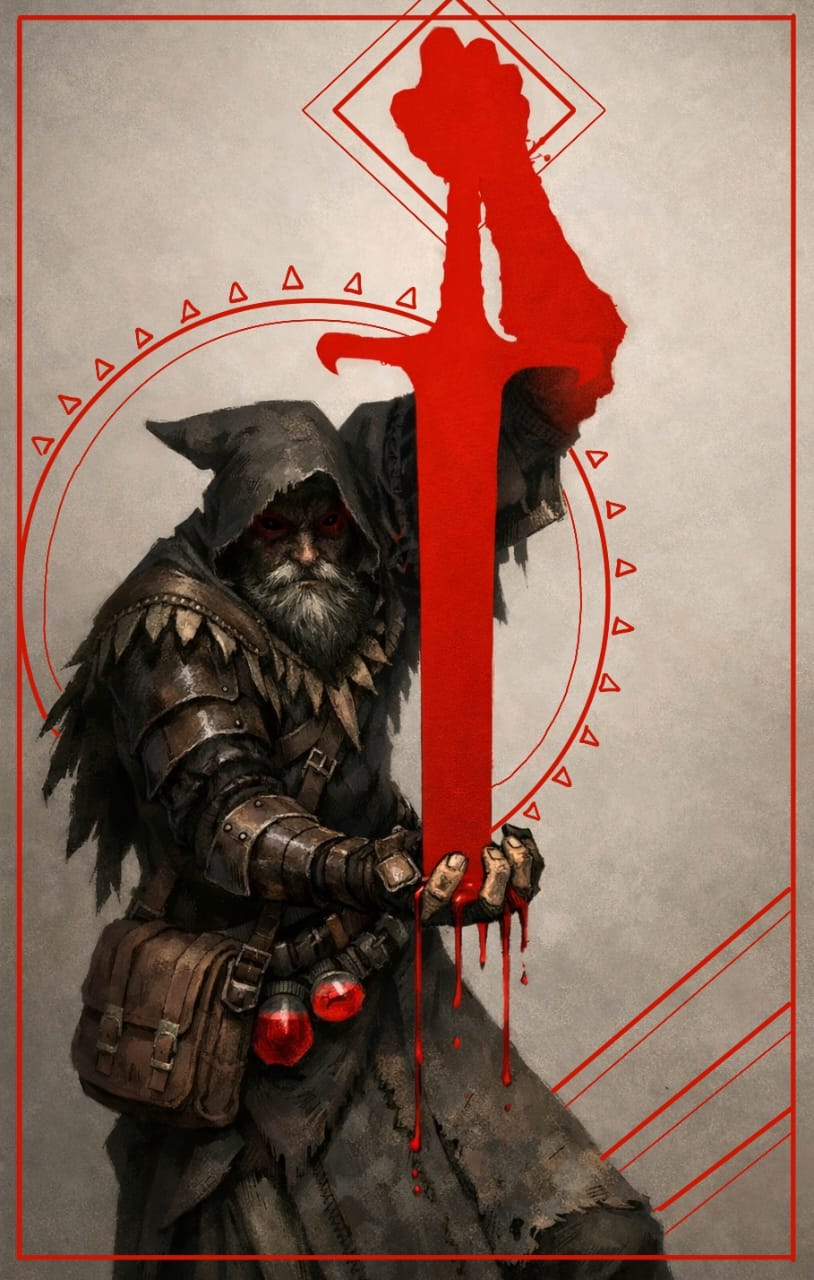
\includegraphics[width=0.75\linewidth]{Images/bloodhunter.jpeg}
    \label{fig:placeholder}
\end{figure}

\begingroup
\DndSetThemeColor[PhbMauve]
\begin{DndSidebar}{Two Halfs of a Whole}
\textit{An organized whole that is perceived as more than the sum of its parts. Wielders of blade \& sorcery...}
\end{DndSidebar}
\endgroup

\subsection{Gestalt Characters}

In this \textit{high-powered campaign variant}, characters essentially \textit{take two classes at every level}, choosing the best aspects of each. The process is similar to multiclassing, except that characters gain the \textbf{full benefits of each class at each level}. if the two classes you choose have aspects that overlap , \textbf{\textit{you choose the better aspect}}.\textbf{\textit{ The gestalt character retains all aspects that don’t overlap.}}

This feature can only be invoked \textbf{at the start of the campaign} and upon the \textbf{Dungeon Master's discretion}. It is required for the party to have \textbf{three or fewer members} generally.

\subsubsection{Hit Dice}
When determining hit die pool and your hit point maximum, you would take whichever hit die would give you the \textbf{most benefit}. For every subsequent level after making your character, look at the two classes you have selected, and \textbf{choose whichever class gives the largest hit die} and add to your hit die pool, and to determine your new Hit Point maximum. Do note that you still only gain \textbf{1 hit die}, and \textbf{1 hit die worth of maximum HP} with a gestalt character.

\subsubsection{Proficiency Bonus}
When determining your proficiency bonus, you still look at your \textbf{current character level} as if you were a non-gestalt character, \textit{as per normal}.

For example a 5th level gestalt character might be a 5th level Fighter and 5th level wizard, but they are still a \textbf{5th level character}.

\subsubsection{Saving Throws}
To determine your\textit{ saving throws}, you do so by taking both starting classes saving throws and \textit{combining those into a list}. You then \textbf{choose two} of those saving throws from that list with which to be proficient in. (IE Fighter/Rogue would \textbf{choose 2 from Str/Dex/Con/Int})

\subsubsection{Class Features}
For Gestalt character, you gain \textbf{all class features \& restrictions} from each of your classes. If your two classes would grant the \textbf{same feature}, such as extra attack, or spell slots, use whichever class which would grant you the \textbf{best bonuses}.

For Example, a Paladin/Sorcerer would determine their spell slots \textbf{as per the Sorcerer spell slot table}. For Example, a Fighter/Barbarian would determine their extra attack from \textbf{Fighter}.

\subsubsection{Spell Casting}

As already stated above, when determining your spell slots you use the class which would give you the \textbf{most spell slots}. The one exception to this is \textbf{Warlocks with any other spell casters}. As warlocks do not gain the "Spell casting" feature and instead get "Pact Magic" a Warlock/Caster would get \textbf{both the spell slots from Warlock and spell slots from the caster}.

When determining which spells you can cast/prepare/know, do so \textit{as written for each class as normal} for your given level. This means that if you have \textbf{two different casters} you would prepare spells for \textbf{both classes as normal}. This in turn grants you a \textit{much wider spell list} from which to choose from over the course of your \textit{"adventuring day"}, but does not grant you \textbf{extra spell slots} (with the above stated exception of warlocks and pact magic).

\subsubsection{Ability Score Improvement}
Ability Score Improvement (ASI for short), has a \textbf{major change} from the normal ruleset when making a Gestalt Character. The ASI's from levels \textbf{4, 8, 12, 16, 19} are \textbf{half as effective}. Meaning that if you wanted to increase your ability scores you would only gain \textbf{1 ASI point} for each "ASI" you would gain at the above levels. If you are using feats you must expend \textbf{BOTH of your ASI's} in order to select a feat.

The exception to this rule is any ASI gained from the \textbf{non-standard list} (\textbf{4, 8, 12, 16, 19}), such as from Fighters levels \textbf{6/14}, or rogues from level \textbf{10}. These "\textit{non-standard}" ASI levels work \textbf{as normal}, granting you \textbf{2 ASI points}, or the ability to select a feat (if allowed in your game).

\begin{figure}[H]
    \centering
    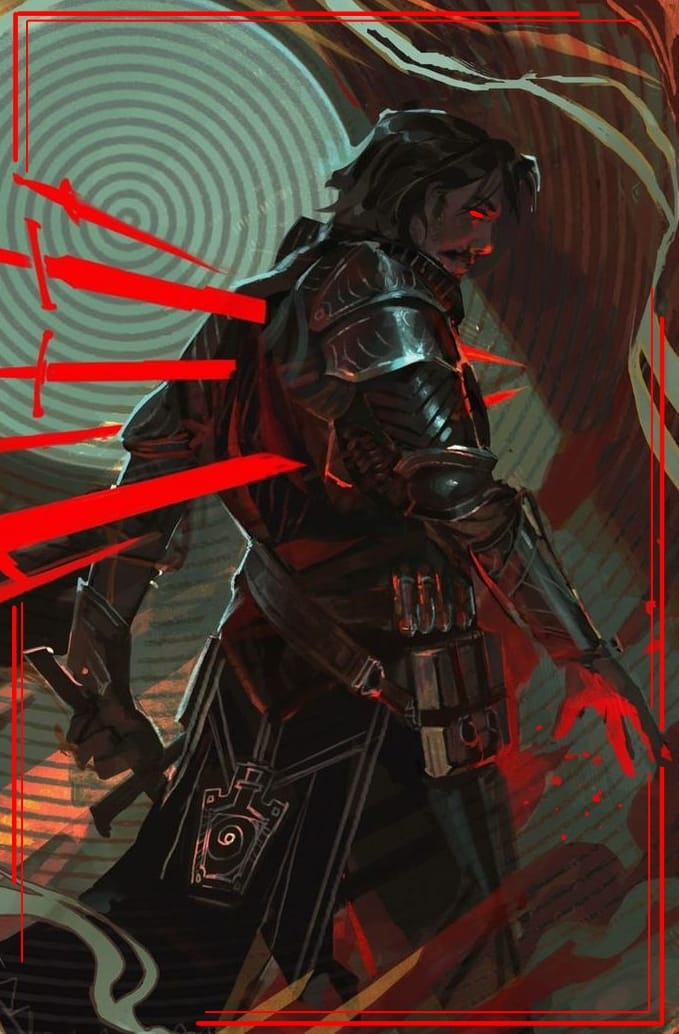
\includegraphics[width=0.7\linewidth]{Images/gestalt.jpeg}
    \label{fig:placeholder}
\end{figure}

\begingroup
\DndSetThemeColor[PhbMauve]
\begin{DndSidebar}{Death is never the end...}
\textit{}
\end{DndSidebar}
\endgroup

\subsection{Heroic Death \& Act of Valour}
These story-driven options to enrich combat do not replace any previous features, yet serve as narrative engines to offer variety to downed party members or avoid TPKs.

\subsubsection{Act of Valour}
Once per campaign, in the place of getting downed at 0 hit points, you can instead opt to\textit{ stand and fight at the cost of all of your inspiration points, regardless of how many you currently have}. 

For three rounds you continue to fight and afterwards you \textit{fall unconscious} and gain the effect:\textit{ Weary}.

You \textit{regain all of your special dice, spell slots and class-specific resources} and any unused features gets depleted again when the effect ends. You can have negative hit points if damage is taken while in this state.

If you are healed by a spell that restores more hit points than your negative hit point value, you do not fall unconscious and continue fighting.

\textbf{Weary:}

Due to fighting past your limits, you are now \textit{dangerously exhausted and have a -4 to all ability checks and attack rolls until your next long rest.}

\subsubsection{Heroic Death}
Once per campaign, irregardless of whether you used the Act of Valour feature, you can choose to keep fighting for 3 rounds after getting downed. You regain all spell slots, class features and special resources as though you were making an Act of Valour.

In addition to this, you add your proficiency bonus to all attack rolls and add it to your spell save DC for the purpose of empowering your spells that require a saving throw. 

You cannot be healed when damage is taken during this state, and you can only be revived with a scroll or spell of true resurrection. 


\subsection{Group Rolls}
When the adventuring party is faced with difficult checks that might not be individually made, the group can add all of their rolls together against a combined DC to utilise everyone's bonus.

\subsubsection{Stealth}
When a party sneaks, instead of individual stealth checks, the whole group rolls and the scores add up to a party sneak score. Failing this ability check, reveals the whole party from stealth. The choice between individual and a group stealth, must be decided and roleplayed beforehand.

\subsubsection{Obstacles}
When the party must overcome obstacles they add all relevant skill check results together against a combined DC to overcome the challenge.

\subsubsection{Bartering}
The whole party barters together using the resultant charisma bonus to skill checks and discounts of the group combined, however the items must be shared and the whole party must unanimously decide to purchase the item.

\begin{DndReadAloud}
    
\end{DndReadAloud}
